% Chapter 5

\chapter{Experiments and Results} % Main chapter title

\label{Chapter5} % For referencing the chapter elsewhere, use \ref{Chapter5}

\lhead{Chapter 5. \emph{Experiments and Results}} % This is for the header on each page - perhaps a shortened title

%----------------------------------------------------------------------------------------

%----------------------------------------------------------------------------------------
There are two principle parts for my experiments. First is to test the EEG data with an autoencoder(didn't add the gradient reversal branch), to see the reconstruction error in order to decide the hidden layer units and other hyper-parameters for training. Second, using all the two sessions EEG data and add the gradient reversal branch to fully built the DANN, and see the performance of the neural network for our objectives.
\section{Architecture of the Neural Network}
For a neural network, first thing how to decide is the architecture of our neural network, as the input layer and output layer architecture have already been fixed(size 56). Two things left to decide:
\begin{enumerate}
	\item Number of hidden layers
	\item Number of units in a hidden layer
\end{enumerate}

As we know, more hidden layers in a neural network will always get better performance like lower mean squared error for reconstruction, but beside, it will always consume more computation time. So choosing the architecture is a trade-off between performance and computation time. In fact, we found that for a architecture with more than one hidden layer, the computation time will be several hours for one training, but we need also to vary the number of hidden units in each layer. In order to do more experiments, we choose at last the architecture like 56-n-56 ($ n \in [1,56] $).

\section{Learning Rate Strategy}
In the training phase of an neural network, the hyper parameter affecting the computation time and the converge speed is the learning rate $ \mu $. The more larger learning rate is, the faster will the neural network trains; the smaller learning rate is, the more accurate the result will be. Instead of setting an constant learning rate, we can adjust the value of learning rate related to the training status. For example, when the error isn't stable, we can set a larger learning rate to accelerate the descent; when the error become stable, we can set a smaller learning rate to let the result more stable.

Tracing the result error with every epoch of training can also help us to determine the maximum iteration needed for converge, so we can find a optimal point between the computation time and the performance.

\subsection{Learning Rate Strategy for Auto-encoder}
For the auto-encoder without the gradient reversal branch, there are several strategy of learning rate strategy proposed by Dr. Sebag and Dr. Gaetan. Which are:
\begin{enumerate}
	\item Exp1: constant learning rate, $ \mu = 0.1 $
	\item Exp2: constant learning rate, $ \mu = 1 $
	\item Exp3: reciprocal of square of epoch number, $ \mu(i_{epoch}) = \frac{1}{\sqrt{i_{epoch}}}$
	\item Exp4: reciprocal of epoch number,  $ \mu(i_{epoch}) = \frac{1}{i_{epoch}} $
	\item Exp5: adaptive learning rate, in this strategy, we will adjust the learning rate by comparing the current loss with previous loss,\begin{itemize}
		\item if the error decreases, multiply the previous learning rate by 1.2
		\item if the error increases, divide the previous learning rate by 2
	\end{itemize}
\end{enumerate}

The result is shown at \fref{fig:3}. The structure of this experiments is 56-5-56, max epoch = 2000, mini-batch size is 50. The training time for each experiment is 40 mins.

The training set we use are example [1,6000] from subject 1 session 1 and valid set are examples [6001,12000]. X axis is the number of epoch and Y axis is the training MSE.

We can see that experiment 1 converges very fast but with a high MSE loss. Experiment 2 are about to converging after 2000 epochs and the MSE loss is small, this looks an good strategy but it takes too much time to converge.

Experiment 3 didn't converge after 2000 epoch and the MSE loss is large. Expriment 4 didn't converge and the MSE loss is average. Experiment 5 which using the adaptive schedule converges after 300 epoch with a very small MSE loss.

From the schema we can tell that the adaptive schedule is the best learning rate strategy because it converges very fast (\textless 300 epochs) and get the smallest MSE loss, except the MSE loss oscillates at the beginning of the training which is normal because the learning rate oscillates a lot at the beginning.
\begin{figure}[htbp]
	\centering
	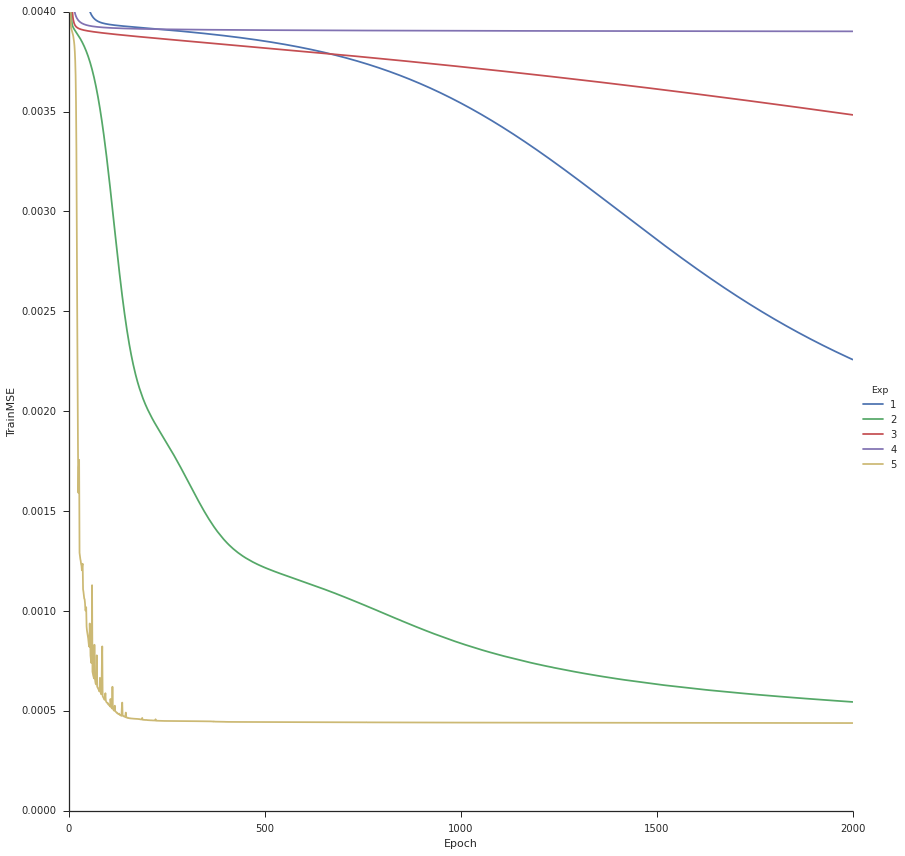
\includegraphics[width=15cm]{Figures/3.png}
	\caption[Train MSE in function with the Epoch number for different learning rate strategy in Auto-encoder]{Train MSE in function with the Epoch number for different learning rate strategy in Auto-encoder}
	\label{fig:3}
\end{figure}
\subsection{Learning Rate Strategy for DANN}
\begin{figure}[htbp]
	\centering
	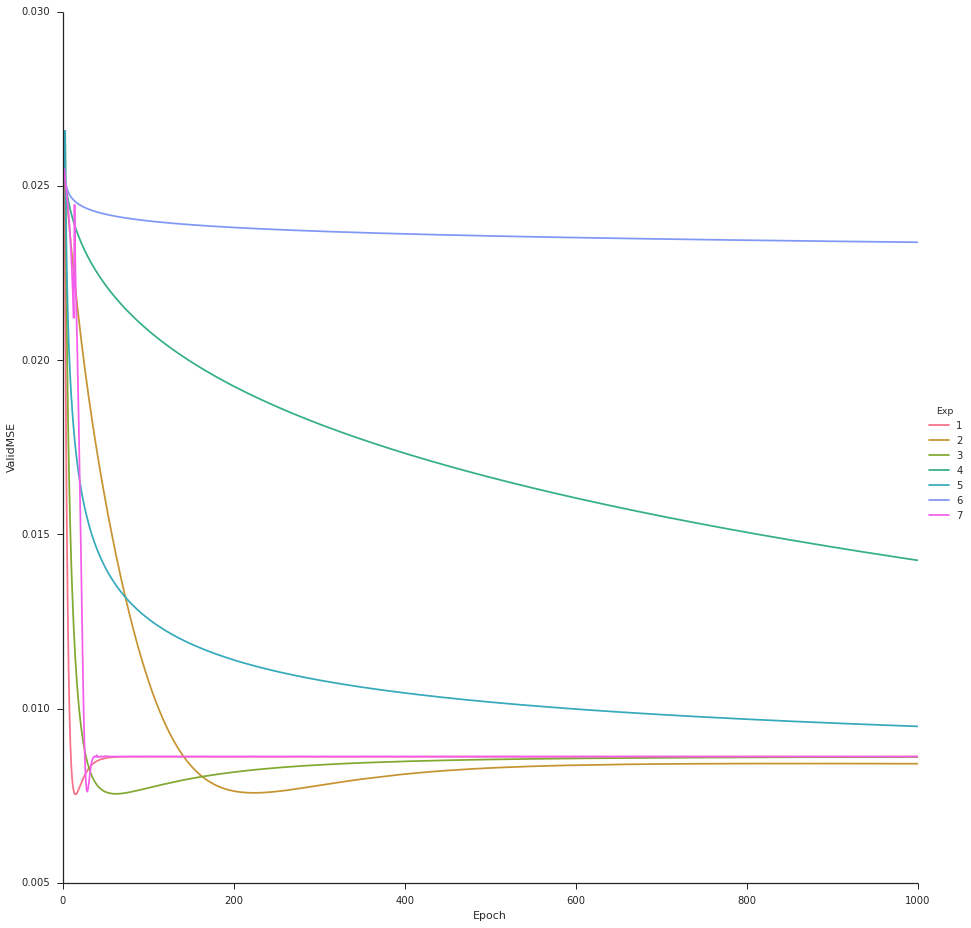
\includegraphics[width=15cm]{Figures/4.png}
	\caption[Train MSE in function with the Epoch number for different learning rate strategy in DANN]{Train MSE in function with the Epoch number for different learning rate strategy in DANN}
	\label{fig:4}
\end{figure}
As the same above, we have also defined several strategy for \textbf{DANN}, those are:
\begin{enumerate}
	\item Exp1: constant learning rate, $ \mu = 1 $
	\item Exp2: constant learning rate, $ \mu = 0.1 $
	\item Exp3: reciprocal of square of epoch number, $ \mu(i_{epoch}) = \frac{1}{\sqrt{i_{epoch}}}$
	\item Exp4: reciprocal of square of epoch number, $ \mu(i_{epoch}) = \frac{0.1}{\sqrt{i_{epoch}}}$
	\item Exp5: reciprocal of epoch number, $ \mu(i_{epoch}) = \frac{1}{\sqrt{i_{epoch}}}$\
	\item Exp6: reciprocal of epoch number, $ \mu(i_{epoch}) = \frac{0.1}{\sqrt{i_{epoch}}}$
	\item Exp7: adaptive learning rate schudule
\end{enumerate}

The results are shown in \fref{fig:4}.


The conclusion is pretty as like in the auto-encoder, adaptive strategy still works the best from all the strategies.

In the following experiments, I will use adaptive strategy in the training phase.
\section{Auto-encoder experiments results}


First experiments is to see the impact of the hidden layer  units for an auto-encoder, results shown at \fref{fig:1} and \fref{fig:2}.
\begin{figure}[htbp]
	\centering
	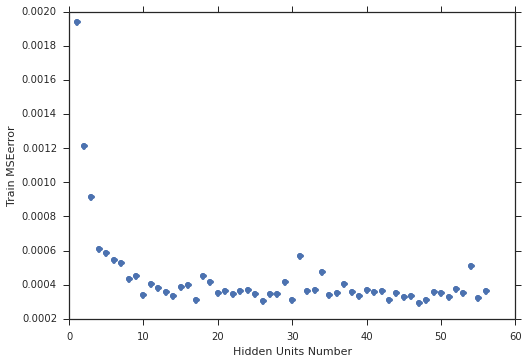
\includegraphics[width=10cm]{Figures/1.png}
	\caption[Train reconstruction error with different hidden layer units]{Train reconstruction error with different hidden layer units}
	\label{fig:1}
\end{figure}
\begin{figure}[htbp]
	\centering
	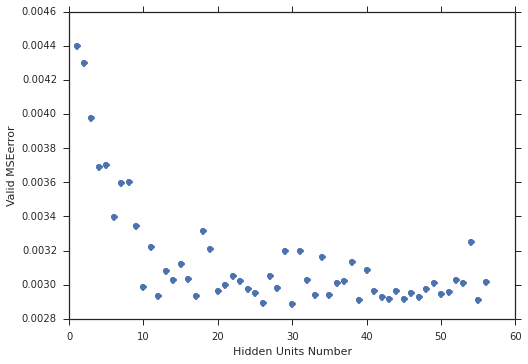
\includegraphics[width=10cm]{Figures/2.png}
	\caption[Valid reconstruction error with different hidden layer units]{Valid reconstruction error with different hidden layer units}
	\label{fig:2}
\end{figure}

This schema gives the MSE error of the auto-encoder with different hidden layer units. The network is trained with mini-batch size=50, learning rate is adaptive, max epoch=1000, structure is 56-n-56.The n I tested varies from 1 to 56. Result is average of 5 runs. The training time for one value of hidden layer units are 50 mins, so the time total used for training is 46 hours.

The training set we use are example[1,6000] from subject 1 session 1 and valid set are examples [6001, 12000] from subject 1 session 1. So in the schema, x axis is the hidden layer units from 1 - 56, on the y axis is the training and valid MSE error.

We can see that the MSE basically decrease when the hidden layer units increases, which is normal for an auto-encoder. Else, we can see before n=8, the error is more large than n>8, which means EEG data is more than 4 dimensions, but the error is basically same if n bigger than 10. For when n=56, ideally, the error should be 0 if we initialize the weight parameters in a matrix like:
\[ 
\begin{pmatrix}
1 & 0 & \cdots & 0 \\
0 & 1 & \cdots & 0 \\
\vdots  & \vdots  & \ddots & \vdots  \\
0 & 0 & \cdots & 1
\end{pmatrix} 
\]

From the results, we can see that it's better to choose the n larger than 10 to ensure that we can reconstruct the initial information from EEG data.

\section{DANN experiments results}
After adding the gradient reversal branch to the auto-encoder, at every back-propagation, the parameters will be updated both by the two branch (label predictor and domain predictor). Label predictor is for minimize the reconstruction loss of the EEG data, where domain predictor is aims at maximizing the domain classification error. So the result will be a trade-off between this two predictor.

Two parameters will be varied in the following experiments:
\begin{itemize}
	\item The number of units in the hidden layer, this parameter helps us to find the optimal architecture of the DANN to balance the computation time and the performance
	\item The parameter lambda $\lambda$ in the gradient reversal layer. $\lambda$ means how much the domain predictor will affect the gradient descent in the back-propagation.
\end{itemize}  

\begin{figure}[htbp]
	\centering
	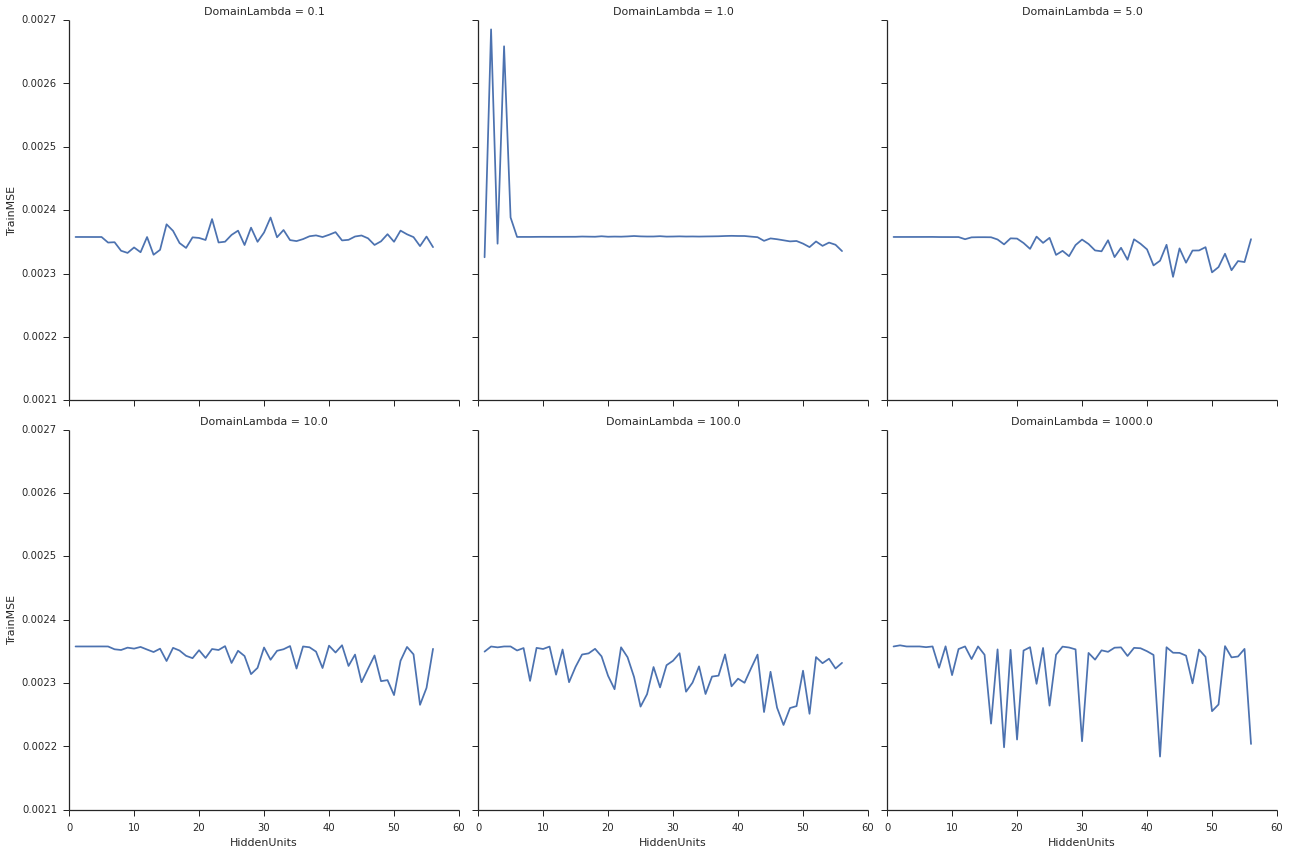
\includegraphics[width=15cm]{Figures/5.png}
	\caption[Train reconstruction error with different hidden layer units in DANN]{Train reconstruction error with different hidden layer units in DANN}
	\label{fig:5}
\end{figure}

\begin{figure}[htbp]
	\centering
	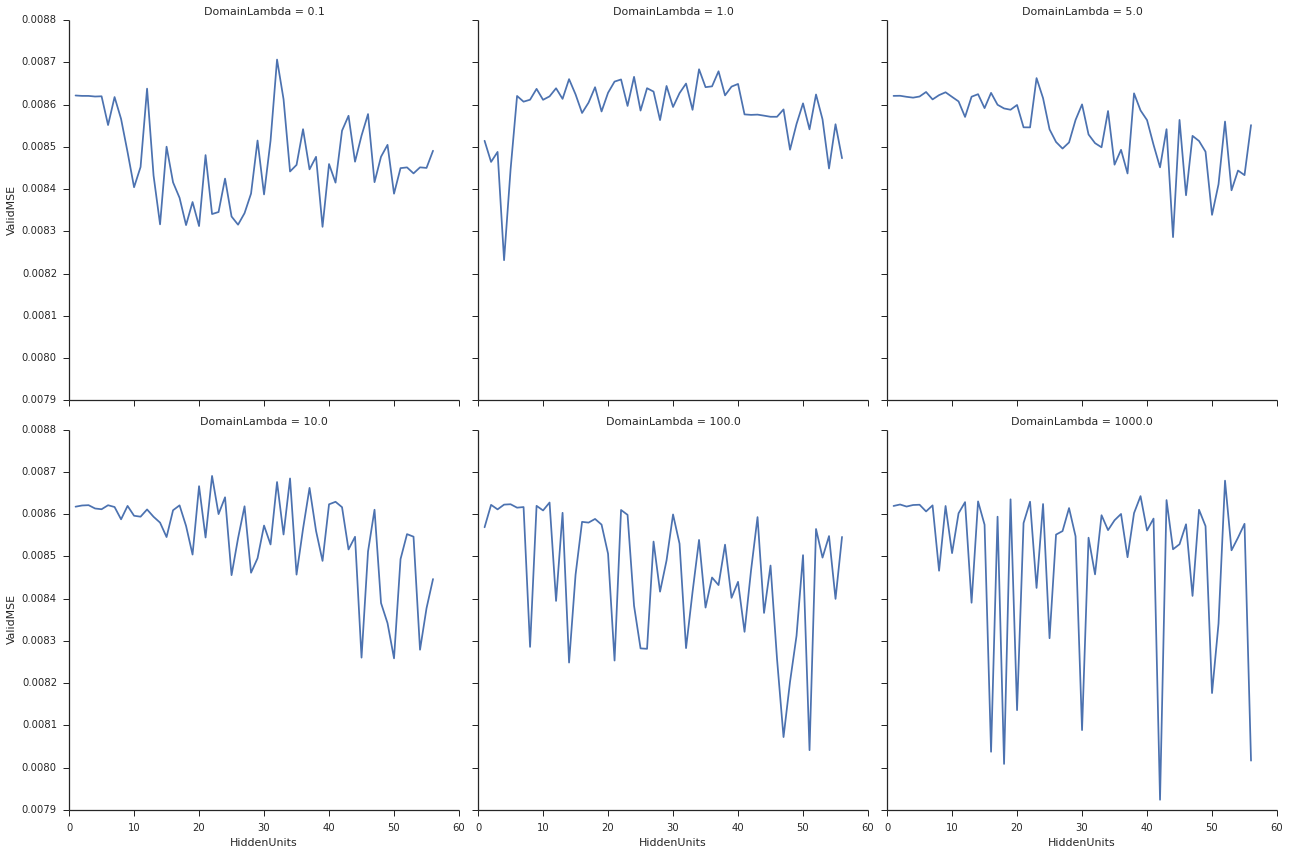
\includegraphics[width=15cm]{Figures/7.png}
	\caption[Valid reconstruction error with different hidden layer units in DANN]{Valid reconstruction error with different hidden layer units in DANN}
	\label{fig:7}
\end{figure}

These schema(\fref{fig:5} and \fref{fig:7}) gives the train and valid reconstruction error with different hidden layer units in DANN. The network is trained with mini-batch size=50, learning rate is adaptive, max epoch=300, structure is 56-n-56.The n I tested varies from 1 to 56. Result is average of 5 runs. The training time for one value of hidden layer units are 70 mins.

The source domain training set we use are example[1,6000] from subject 1 session 1 and valid set are examples [6001, 12000] from subject 1 session 1. The target domain training set are examples [1,6000] from subject 1 session 2, valid set are examples [6001, 12000] from subject 1 session 2.In the schema, x axis is the hidden layer units from 1 - 56, on the y axis is the training and valid MSE error.

For $\lambda = 1$, the MSE loss is pretty stable except when $n \in [1,8]$. With the value of $\lambda$ increases, the MSE loss become more oscillated. But the base losses are basically the same, when the hidden layer units number are large, it can sometimes reach a smaller MSE loss. In our inference, the MSE loss should decreases with the hidden layer units increases, the result didn't totally accord with our inference but shows the same tendency. 

\begin{figure}[htbp]
	\centering
	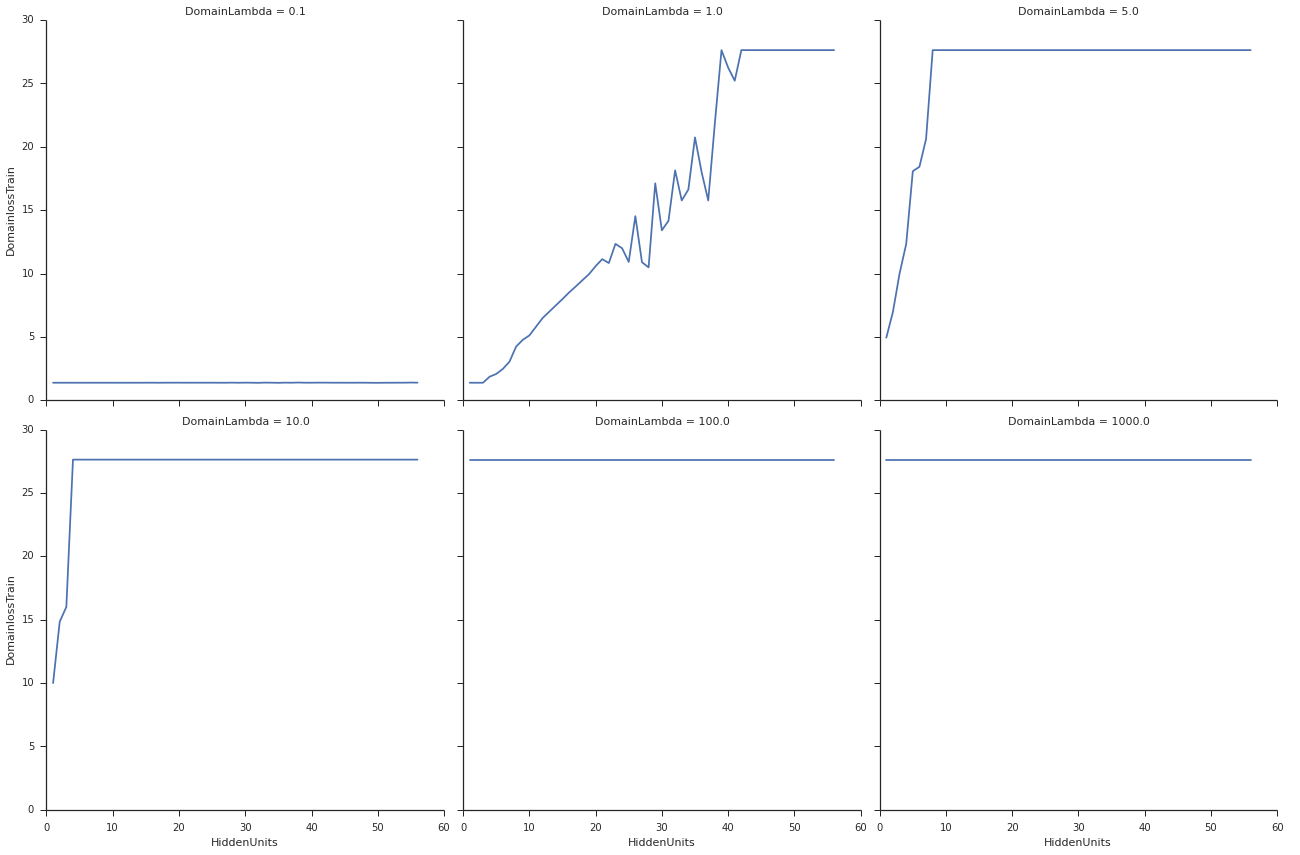
\includegraphics[width=15cm]{Figures/8.png}
	\caption[Train Domain BCE loss with different hidden layer units in DANN]{Domain BCE loss with different hidden layer units in DANN}
	\label{fig:6}
\end{figure}
\begin{figure}[htbp]
	\centering
	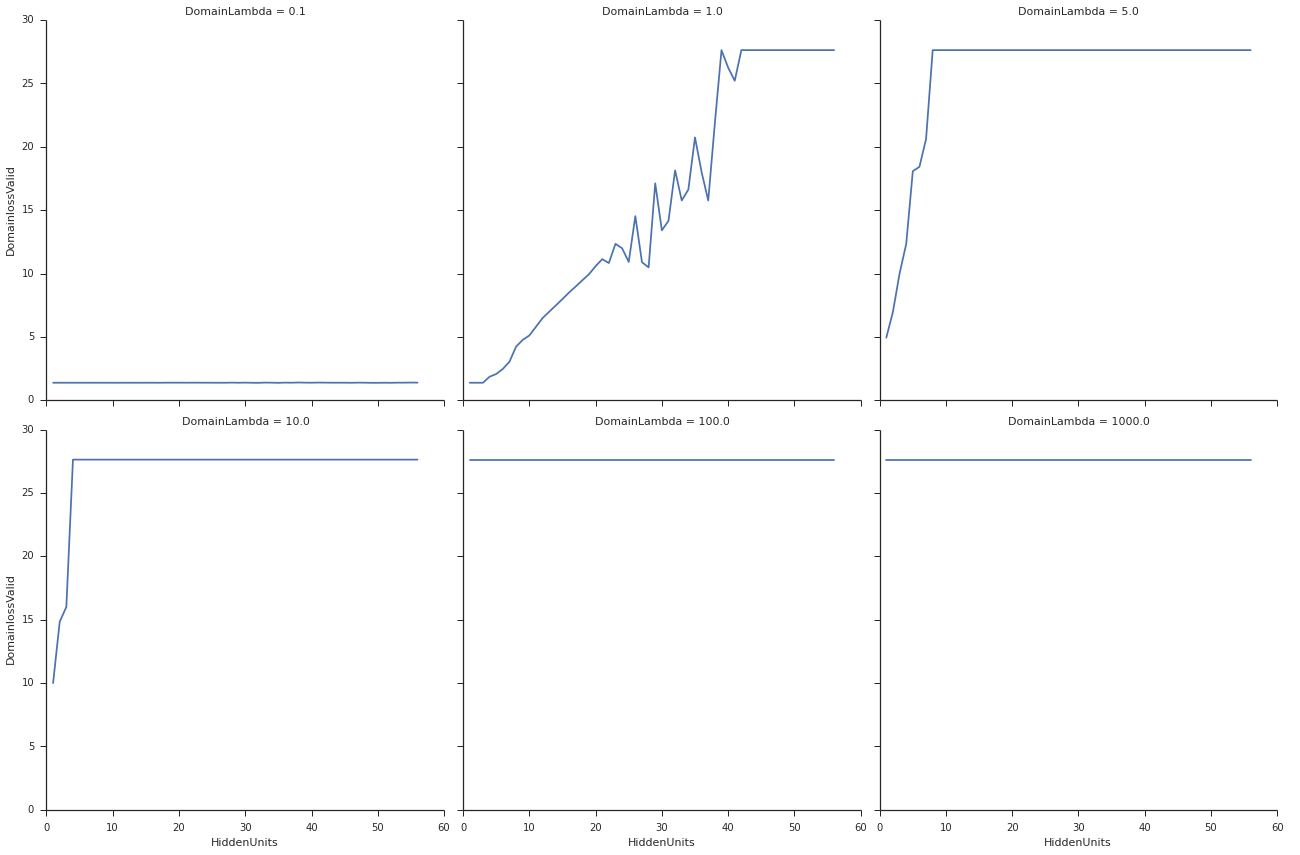
\includegraphics[width=15cm]{Figures/6.png}
	\caption[Valid Domain BCE loss with different hidden layer units in DANN]{Domain BCE loss with different hidden layer units in DANN}
	\label{fig:8}
\end{figure}

These schema(\fref{fig:6} and \fref{fig:8}) gives the train and valid domain BCE loss with different hidden layer units in DANN. The network is trained with mini-batch size=50, learning rate is adaptive, max epoch=300, structure is 56-n-56.The n I tested varies from 1 to 56. Result is average of 5 runs. The training time for one value of hidden layer units are 70 mins.

The source domain training set we use are example[1,6000] from subject 1 session 1 and valid set are examples [6001, 12000] from subject 1 session 1. The target domain training set are examples [1,6000] from subject 1 session 2, valid set are examples [6001, 12000] from subject 1 session 2.In the schema, x axis is the hidden layer units from 1 - 56, on the y axis is the training and valid MSE error.

For $\lambda = 1$, the domain BCE loss is positively correlated with the hidden layer units. When the $\lambda$ increases from 1 to 1000, the domain BCE loss become more stable regarding the hidden units number. That is to say the influence of the architecture become smaller. When the domain BCE loss become 27, than means the domain classifier has a high error rate, so that EEG data from the two sessions become indiscriminate which is our purpose.